\section{Streamlining the build process}
Before this project began PIPE 4's build process was hosted on SourceForge and made use of CVS for its version control. In line with modern practice we migrated the project to Git and transferred the project from SourceForge to GitHub because it provides a richer variety of developer tools including issue tracking, forking, easy releases, continuous-integration and the support of a project website.

% \begin{figure}[tb]
% \begin{center}
%     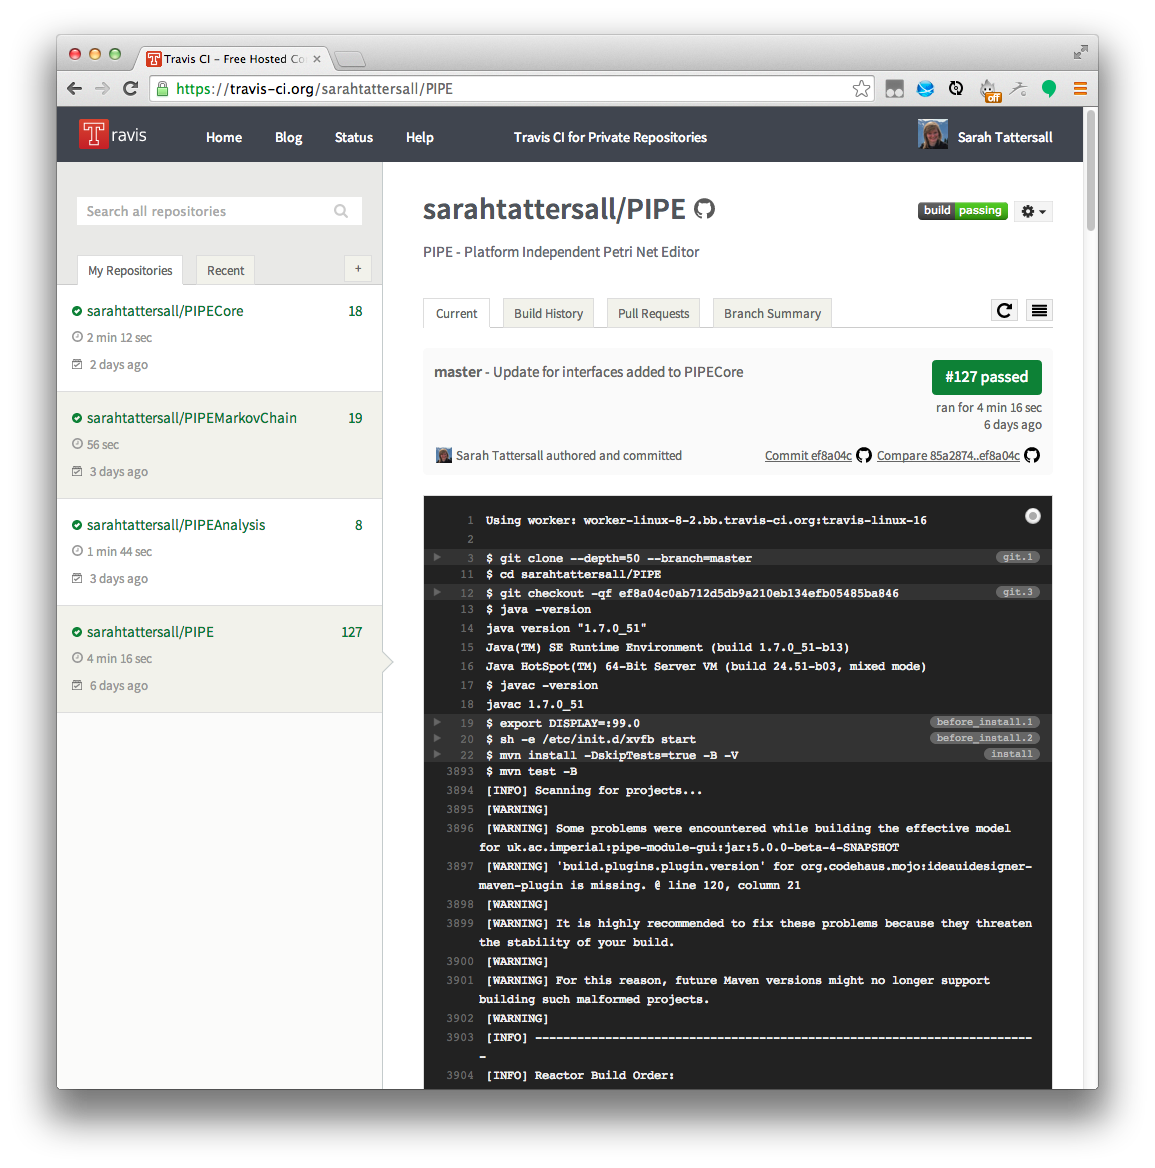
\includegraphics[width=\linewidth]{build/travis_ci.png} 
%     \caption{Originally there was no continuous integration server for PIPE 4 which meant that committed changes that broke the build could go undetected. This figure shows the continuous integration server, Travis CI, set up for PIPE 5. The entire console output is shown in the build which is particularly helpful for spotting the cause of an error in failing builds. Builds on Travis CI are triggered by post-commit hooks when pushing changes to GitHub.}
%     \label{fig:travis_ci}
% \end{center}
% \end{figure}

Beyond this we set up a Maven build-system for PIPE 5 to provide a stable cross-platform build process and dependency management system. This overcame problems caused by a collection of user-written build scripts and removed the need to ship external libraries with the codebase.

We made use of Maven build plug-ins to simplify the full release process of PIPE 5 which now involves: (i) Resolving any SNAPSHOT dependencies, (ii) bumping the version number, (iii) creating a runnable uber-jar, (iv) deploying a project to a Maven repository as an artifact, (v) generating a GitHub release. The command to execute all of the aforementioned steps can be performed in a single line, which significantly eases the build and release process of PIPE 5:
\begin{lstlisting}
   mvn release:clean release:prepare release:perform.
\end{lstlisting}

Finally we set up a continuous integration server using Travis CI for PIPE 5. Builds on the server are triggered via post-commit hooks on GitHub and the most recent build status is shown on the GitHub landing page.
\clearpage